\documentclass[10pt]{article}

\usepackage{draftcopy}
\usepackage{multirow}
\usepackage{rotating,graphicx}
%\usepackage{wrapfig}
\usepackage{amssymb}
\usepackage{amsmath}
\usepackage{lscape}
\usepackage{times}
\usepackage{color}  % For \textcolor and \color % Ex. : \textcolor{red}{Text colored with} ; {\color{red}Text colored with}
\usepackage{soul}   % For \hl{ highlighted text} ; \sethlcolor{colorname}
%\usepackage[table]{xcolor}
\usepackage{xcolor,colortbl}
\usepackage{capt-of}
\usepackage{textcomp}  % allows \textonehalf,  \textonequarter, or else
%\usepackage{mathcomp}  % make it math compatible

\oddsidemargin =-0.6in
\evensidemargin=-0.6in
%\textwidth=7.6in   % owl
 \textwidth=7.8in % laptop
\textheight=10.2in
% \topmargin=-.25in   % owl
 \topmargin=-1.in    % laptop
\footskip=-.0in

\newcommand{\Bl}{\ensuremath{B_{{low}}}}
\newcommand{\Bh}{\ensuremath{B_{{high}}}}
\newcommand{\Il}{\ensuremath{I_{{low}}}}
\newcommand{\Ih}{\ensuremath{I_{{high}}}}
\newcommand{\Br}{\ensuremath{B\! \rho}}
\newcommand{\CE}{concentration ellipse}
\newcommand{\CES}{CE-$\rm \mathcal{S}$}
\newcommand{\dEE}{\small \ensuremath{\frac{dE}{E}}}
\newcommand{\eg}{\ensuremath{\it e.g.}}
\newcommand{\Ha}{\ensuremath{\mathcal{H}}}
\newcommand{\Sa}{\ensuremath{\mathcal{S}}}
\newcommand{\vs}{\ensuremath{\it vs.}}
\newcommand{\ie}{\ensuremath{\it i.e.}}
\newcommand{\hbrk}{\hfill \break}
\newcommand{\sr}{synchrotron radiation}
\newcommand{\SRl}{SR loss}
\newcommand{\x}{\ensuremath{x}} 
\newcommand{\xp}{\ensuremath{{x'}}}
\newcommand{\z}{\ensuremath{z} }
\newcommand{\zp}{\ensuremath{{z'}}}
\newcommand{\y}{\ensuremath{y} }
\newcommand{\yp}{\ensuremath{{y'}}}
\newcommand{\dl}{\ensuremath{{\delta l}}} 
\newcommand{\dE}{\ensuremath{{\delta E}}}
\newcommand{\X}{\ensuremath{X} }
\newcommand{\Xp}{\ensuremath{{X'}}}
\newcommand{\Z}{\ensuremath{Z} }
\newcommand{\zg}{Zgoubi}
\newcommand{\Zp}{\ensuremath{{Z'}}}
\newcommand{\Y}{\ensuremath{Y} }
\newcommand{\Yp}{\ensuremath{{Y'}}}
\newcommand{\Len}{\ensuremath{l} }
\newcommand{\Mom}{\ensuremath{E}}
\newcommand{\Sx}{\ensuremath{\mathcal{S}_x}}
\newcommand{\Sy}{\ensuremath{\mathcal{S}_y}}
\newcommand{\Sz}{\ensuremath{\mathcal{S}_z}}

\newcommand{\C}{\ensuremath{\mathcal{C}}}
\newcommand{\D}{\ensuremath{\mathcal{D}}}
\newcommand{\HH}{\ensuremath{\mathcal{H}}}
\newcommand{\bHH}{\bar \HH}
\newcommand{\com}{{center of mass}}
\newcommand{\lab}{{laboratory frame}}
\newcommand{\LL}{\ensuremath{\mathcal{L}}}
\newcommand{\rms}{\ensuremath{rms}}
\newcommand{\wrt}{{with respect to}}

\newcommand{\bull}{\ensuremath{\bullet~}}
\newcommand{\cf}{\ensuremath{\textsl{cf.}}}
\newcommand{\bhel}{\ensuremath{\mathbf{^3He^{2+}}}}
\newcommand{\hel}{\ensuremath{\mathrm{^3He^{2+}}}}
\newcommand{\nib}{\noindent \ensuremath{\bullet~}}
\newcommand{\snib}{\noindent {\small \ensuremath{\bullet~}}}
\newcommand{\nid}{\noindent \ensuremath{\diamond~}}
\newcommand{\snid}{\noindent {\small \ensuremath{\diamond~}}}
\newcommand{\nin}{\noindent~}
\newcommand{\no}{\ensuremath{\mathbf{\vec n_0}}}
\newcommand{\MC}{Monte~Carlo}
\newcommand{\p}{\ensuremath{\mathbf{p}}}
\newcommand{\pp}{$\rm p\! \! \uparrow$}

\definecolor{orange}{rgb}{1,0.5,0}
\definecolor{yelloworange}{rgb}{1,.647,0}
\newcommand{\black}{\color{black}}
\newcommand{\red}{\color{red}}
\newcommand{\green}{\color{green}}
\newcommand{\blue}{\color{blue}}
\newcommand{\yo}{\color{yelloworange}}

\newcommand{\referenceA}{\rm  }
\newcommand{\referenceB}{\rm }
\newcommand{\referenceC}{\rm }

\pagestyle{headings}
\markboth{\small  \referenceA ~ ~   \referenceB ~ ~  \referenceC \hfill }
         {\small  \referenceA ~ ~   \referenceB ~ ~  \referenceC \hfill }


\begin{document}

\thispagestyle{empty}

\begin{minipage}{1.\linewidth}
\bf
  \flushright{F. M\'eot}
\vspace{-2ex}
  
  \flushright{BNL C-AD}
\vspace{-2ex}
  
  \flushright{Zgoubi 2019 Workshop, Boulder, CO}
\vspace{-2ex}
  
\flushright{24-29 Aug. 2019} 
\end{minipage}


\vspace{5ex}

\centerline{\LARGE \bf
  An Introduction to  ``WIENFILTER'' 
}

~

\centerline{\LARGE \bf
Exercise 1: A Parallel Plate Electrostatic Deflector
}


\section*{Recommended readings}

\nin - Section  "3.1 - Wien filter"  in 
``Generalization of the Zgoubi method for ray-tracing to include electric fields'', \\
../../documentation/electrificationOfZgoubi.pdf

\smallskip
\nin - Zgoubi Users' Guide, regarding the keywords used in the exercise (WIENFILTER, OBJET/KOPT=2, OPTIONS/CONSTY, SEPARA in question 6/, etc.). Hint: use the index (last 3 pages of the Guide) to locate the related sections in Part~A and Part~B. 


\smallskip
\nin - During the exercise, it is recommended to keep 2 copies of the guide at hand, with one copy opened at the Index (last 3 pages of the document).

\section*{Keywords we play with in this exercise}

\texttt{WIENFILTER} is the optical element used  (pp.~168 and 306 in the Users' Guide), with B=0  so that it operates as a simple parallel plate electrostatic deflector.

\nin Note: \texttt{ELMIR, ELMIRC} and even \texttt{ELMULT} or \texttt{EBMULT}  could be used as well, they would be able to provide this dipole $ \vec E$ field simulations (see "Optical elements versus keywords'' in the Users' Guide).


\section*{Working hypotheses}

\nib The Wien filter length is $ L$. Take $ \vec E =\vec E_Y \parallel \vec Y$.
Take  hard-edge E-field model  so to allow tight comparison with theory\footnote{G.\,Leleux, INSTN Saclay, 1978 (unpublished)}.

\nib In order to check numerical outcomes, the following can be used:

\begin{minipage}{.69\linewidth}
\nin - The expected trajectory is a catenary with equation
%  
$$ Y_{th}(X) = \frac{E_i}{qE_Y} \left( \cosh \dfrac{qE_Y X}{\beta_i E_i } -1 \right)$$
with $E_i$  initial total energy, $c\beta_i$ initial velocity, $q$  particle charge

~

\nin -  Spin rotation: assume we manage to maintain $\vec E \perp \vec v$, namely, $\vec v = v_X$, always. Thus expected spin rotation over L  is (Eq.\,2.1.4 in Zgoubi Users' Guide)
$$ \theta_s = (a\gamma+\dfrac{\gamma}{1+a\gamma})\beta_X^2 \dfrac{E_YcL}{B\rho}  $$

\end{minipage} \hfill
\begin{minipage}{.3\linewidth}
  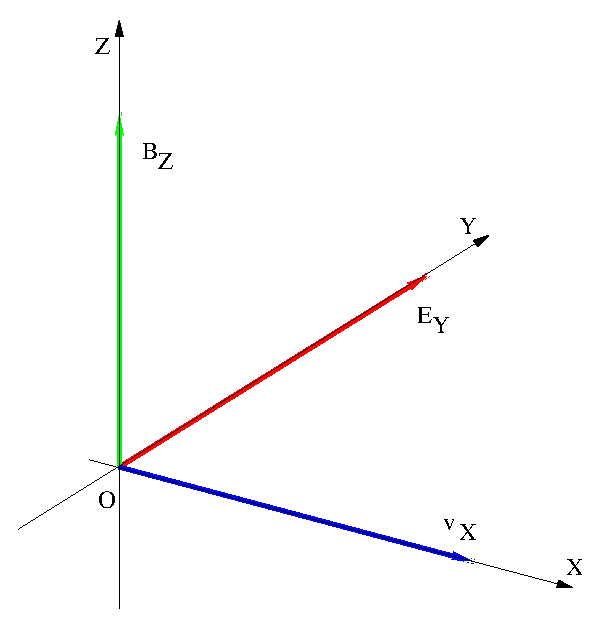
\includegraphics[width=0.75\linewidth]{wienF.eps}
\end{minipage}


\section*{ Numerical experience }


\nin 1/ Let's  first walk through the fortran, see what happens when the execution pointer meets 'WIENFILTER'  in zgoubi.dat sequence...

\begin{itemize}
\item Open zgoubi\_main.f : it calls zgoubi. The rest of the it essentially manages the 'FIT' procedure.
\item Open zgoubi.f 
\begin{itemize}
  \item find include/LSTKEY.H: take a look into it, spot WIENFILTER -~and all of zgoubi keywords! If you need to add a keyword, that's here
  \item find 'CALL RWIENF', look into rwienf.f. What does it do?
  \item it is followed by'CALL QUASEX'. 
    Optical elements call either QUASEX, or AIMANT (check that statement, scrolling through zgoubi.f), what's the difference between the two? 
  \item  Open quasex.f.   In there, find 'CALL CHXC'. What does it do? 
  \begin{itemize}
    \item open chxc.f
    \begin{itemize}
      \item find WIENF therein. Open wienfi.f, take a look to the various ``data initializations'' necessary prior to tracking
      \end{itemize}
    \item find 'CALL TRANSF' in quasex, open transf.f: it pushes the particles, one by one, through 'INTEGR'
    \begin{itemize}
      \item find 'CALL INTEGR', open integr.f: it pushes a particle, step by step, 
        through WIENF (or any other element)
      \item In integer.f look for 
        (i) 'CALL CHAMC',
          (ii) 'CALL CHAMK', 
          (iii) 'CALL DEVTRA': 
          Figure out what each does.
    \end{itemize}
  \end{itemize}
\end{itemize}
\end{itemize}

~

\nin 2/ Set up a Wien filter sequence with $ E_Y=0.98$\,MV/m,  $ L=0.5$\,m.
Consider an electron with 350\,keV energy\footnote{Data after E. Wang, see documentation in exercise 2}. 

 Run that sequence and check (in zgoubi.res)  final $Y(X\equiv L)$,  particle deviation, compare with result from catenary equation above.

~

\nin 3/ Check the effect of step size:

Using REBELOTE, get a scan of Y values for $ \Delta s = .001:10$\,cm.
   Plot $(Y-Y_{th})/Y_{th}$ versus step size (can use gnuplot to plot data read from zgoubi.fai).

   ~

   \nin 4/
   Force Y=0 across the Wien filter, by means of OPTIONS/CONSTY.

   Check the rotation of an initial $\vec S \equiv \vec S_X$, at the downstream end of the condenser (X=L), compare to expected $\theta_s$. 

Check convergence of result versus integration step size. 
   
   ~

   \nin 5/ Check SEPARA keyword in Zgoubi Users' Guide. What is the difference in SEPARA method, compared to WIENFILTER?

Try it and compare with WIENFILTER outcomes in questions 2/ and 3/.
  
   ~

   \nin 6/ Add fringe-fields.

   3.a  Plot the particle trajectory and the $E_Y$ and $B_Z$ fields along the trajectory.

   3.b  Plot particle energy versus distance, conclude on the importance of fringe fields as to 6-D symplecticity. 




   \end{document}
